\hypertarget{comparative-evaluation-of-gmm-guided-motion-planning-samplers}{%
\section{Comparative evaluation of GMM-guided motion-planning samplers}\label{comparative-evaluation-of-gmm-guided-motion-planning-samplers}}

\hypertarget{experimental-design}{%
\subsection{Experimental design}\label{experimental-design}}

We compared two methods for incorporating a deformed task-parameterized Gaussian mixture model (TP-GMM) into RRTConnect: Cartesian sampling followed by inverse kinematics (Cartesian + IK), and local projection into joint space (joint projection). An unrestricted OMPL joint-space sampler provided a reference configuration. All three used the same robot model, collision scene, complete start configuration and joint-space goal within each environment, with a single planning attempt and a 3 s planning budget. Path simplification was disabled. The objective was to characterize the tradeoffs among the implemented sampling configurations before evaluation on the EV battery-disassembly benchmark.

The evaluation comprised 120 environments from a Panda table-and-cylinder task family. Three obstacle-layout strata and two normalized RL clearance inputs, 0.2 and 0.8, were balanced within each of two 60-environment cohorts. The first cohort used ten repeats per method and the second five, yielding 900 requests per method and 2,700 requests overall. The table surface was fixed at z = 0.25 m, with goal heights between 0.45 and 0.54 m. Each environment supplied a shared TP-GMM reproduction and RL-deformed model to both GMM samplers. Sampler order was randomized within repeats. Custom sampler seeds were recorded, although OMPL and IK retained independent internal random streams.

Both GMM samplers used covariance-based truncation with Mahalanobis cutoff 3.0. For a selected component \(k\), Cartesian + IK draws a spatial target

\[x = \mu_k + L_k z,\qquad z\sim\mathcal{N}(0,I_3)\mid\lVert z\rVert\leq3,\]

where \(L_kL_k^T=\Sigma_k\) after the numerical covariance floor, and component selection follows the normalized mixture weights. Each target is converted into a robot configuration by IK with a randomized initial guess and configured orientation bias. Joint projection first constructs diverse IK anchors near component means. Around an anchor \(q_k\), it proposes

\[q = q_k + A_kL_kz + \sigma_N Z_k u,\qquad u\sim\mathcal{N}(0,I),\]

where \(A_k\) is a right inverse of the translational Jacobian and \(Z_k\) spans its null space. Joint bounds, a trust region, nonlinear FK support, linearization residual and collision/constraint checks filter the proposals. The joint-space proposal is therefore a local approximation, while Cartesian targets follow the truncated spatial mixture before IK and validity conditioning. Neither method's accepted robot configurations should be interpreted as unconditioned GMM draws.

The covariance eigenvalue floor was \(10^{-8}\) m\(^2\). Projection used at most three anchors per component from sixteen nominal IK attempts, a 5 ms per-call IK budget, null-space standard deviation 0.08 rad, a maximum joint-displacement norm of 0.6 rad and a 0.01 m linearization-residual tolerance. The model and RL policy were fixed across methods and environments; only their environment-conditioned reproduction and deformation varied.

Both custom methods used the same hard positional corridor, represented by a union of oriented boxes enclosing the cutoff ellipsoids. Uniform planner-state fallback and online Cartesian rescue in the projected method were disabled. Randomized IK initialization remained part of the IK procedure. Unrestricted OMPL sampled the bounded joint space with no GMM corridor and required no GMM/RL preparation. Consequently, its comparison with the GMM methods measures complete planning configurations with different allowed regions, rather than isolating proposal density alone. The GMM methods also differ in orientation behavior; translational null-space motion does not preserve tool orientation, and no hard path-orientation constraint was imposed.

A request was successful only if planning succeeded and the returned path passed a dense audit of bounds, feasibility, collisions and applicable constraints. The audit interpolated at joint-group distance increments of at most 0.01. Failed planning and rejected returned paths remained in the success denominator. Joint travel used MoveIt's joint-group distance metric; end-effector length and minimum padded robot-to-world clearance were measured along audited paths. End-effector-to-cylinder clearance was reported separately. These sampled clearance metrics are distinct from the normalized RL clearance input and do not certify continuous collision freedom.

The environment was the statistical unit. Each environment received equal weight despite the cohorts' different repeat counts. Paired method differences were averaged over repeats within each environment, with path-quality comparisons restricted to repeat pairs that succeeded under both methods. We used 20,000 cluster-bootstrap resamples stratified by cohort, obstacle layout and requested clearance, and two-sided environment-level sign-permutation tests with 100,000 draws or exact enumeration when applicable. All 24 pairwise tests across eight outcomes shared one Holm correction. Confidence intervals are pointwise 95\% intervals. This combined analysis is retrospective: the configuration was selected during preliminary diagnostic work on these environments, so these results are not an independent confirmatory test.

\hypertarget{results}{%
\subsection{Results}\label{results}}

All methods achieved high observed audited success (Table 1). Cartesian + IK succeeded in 899/900 requests, joint projection in 897/900, and unrestricted OMPL in 900/900. Cartesian had one returned-path audit rejection; projection had two audit rejections and one planning failure. Each audit rejection contained a sampled collision and counted as a failure. No pairwise success-rate difference was supported after correction. This absence of a detected difference does not establish equivalence, and OMPL's complete observed success does not imply perfect population reliability. The sampler records confirmed zero uniform fallback attempts, zero missing-anchor rescues and zero projected online IK calls.

Table 1. Observed successes and environment-weighted mean performance. Path metrics average successful requests within each environment. Raw success percentages pool requests and therefore use different weights from the environment-level estimates. Pipeline latency is attributed as described below.

\begin{longtable}[]{@{}
  >{\raggedright\arraybackslash}p{(\columnwidth - 14\tabcolsep) * \real{0.0968}}
  >{\raggedleft\arraybackslash}p{(\columnwidth - 14\tabcolsep) * \real{0.1290}}
  >{\raggedleft\arraybackslash}p{(\columnwidth - 14\tabcolsep) * \real{0.1290}}
  >{\raggedleft\arraybackslash}p{(\columnwidth - 14\tabcolsep) * \real{0.1290}}
  >{\raggedleft\arraybackslash}p{(\columnwidth - 14\tabcolsep) * \real{0.1290}}
  >{\raggedleft\arraybackslash}p{(\columnwidth - 14\tabcolsep) * \real{0.1290}}
  >{\raggedleft\arraybackslash}p{(\columnwidth - 14\tabcolsep) * \real{0.1290}}
  >{\raggedleft\arraybackslash}p{(\columnwidth - 14\tabcolsep) * \real{0.1290}}@{}}
\toprule\noalign{}
\begin{minipage}[b]{\linewidth}\raggedright
Method
\end{minipage} & \begin{minipage}[b]{\linewidth}\raggedleft
Audited success
\end{minipage} & \begin{minipage}[b]{\linewidth}\raggedleft
Action time (ms)
\end{minipage} & \begin{minipage}[b]{\linewidth}\raggedleft
Attributed pipeline (ms)
\end{minipage} & \begin{minipage}[b]{\linewidth}\raggedleft
PAR2 (ms)
\end{minipage} & \begin{minipage}[b]{\linewidth}\raggedleft
Joint travel (rad)
\end{minipage} & \begin{minipage}[b]{\linewidth}\raggedleft
EE length (m)
\end{minipage} & \begin{minipage}[b]{\linewidth}\raggedleft
Robot--world clearance (mm)
\end{minipage} \\
\midrule\noalign{}
\endhead
\bottomrule\noalign{}
\endlastfoot
Cartesian + IK & 899/900 (99.89\%) & 150.94 & 179.66 & 155.80 & 10.847 & 0.853 & 21.694 \\
Joint projection & 897/900 (99.67\%) & 158.90 & 187.71 & 178.36 & 9.645 & 0.788 & 20.156 \\
OMPL unrestricted & 900/900 (100\%) & 167.25 & 168.74 & 167.25 & 13.820 & 2.218 & 25.490 \\
\end{longtable}

Joint projection produced shorter paths than Cartesian + IK on the 896 repeat pairs successful under both methods, covering all 120 environments. Its mean reduction in joint travel was \textbf{1.194 rad} (95\% CI 0.826--1.563; Holm-adjusted \(p<0.001\)), and its mean reduction in end-effector path length was \textbf{0.0643 m} (95\% CI 0.0389--0.0901; adjusted \(p<0.001\)). The direction of both effects was consistent across the two cohorts. This is the strongest evidence favoring one GMM sampler over the other in the present study. It concerns unsimplified successful paths and does not establish path optimality or an execution-time advantage.

Both GMM configurations also produced shorter paths than unrestricted OMPL. On matched successful requests, the joint-travel reductions were 2.972 rad for Cartesian + IK and 4.177 rad for projection; the corresponding end-effector length reductions were 1.364 m and 1.430 m. All four comparisons had adjusted \(p<0.001\). These gains coexist with the GMM corridor restriction and should not be attributed solely to a more efficient sampling distribution. Unrestricted OMPL achieved greater minimum robot-to-world clearance, by 3.831 mm relative to Cartesian + IK and 5.336 mm relative to projection (both adjusted \(p<0.001\)). Between the GMM samplers, the clearance differences were not supported after correction: adjusted \(p=0.411\) for robot-to-world clearance and \(p=0.062\) for end-effector-to-cylinder clearance.

\begin{figure}
\centering
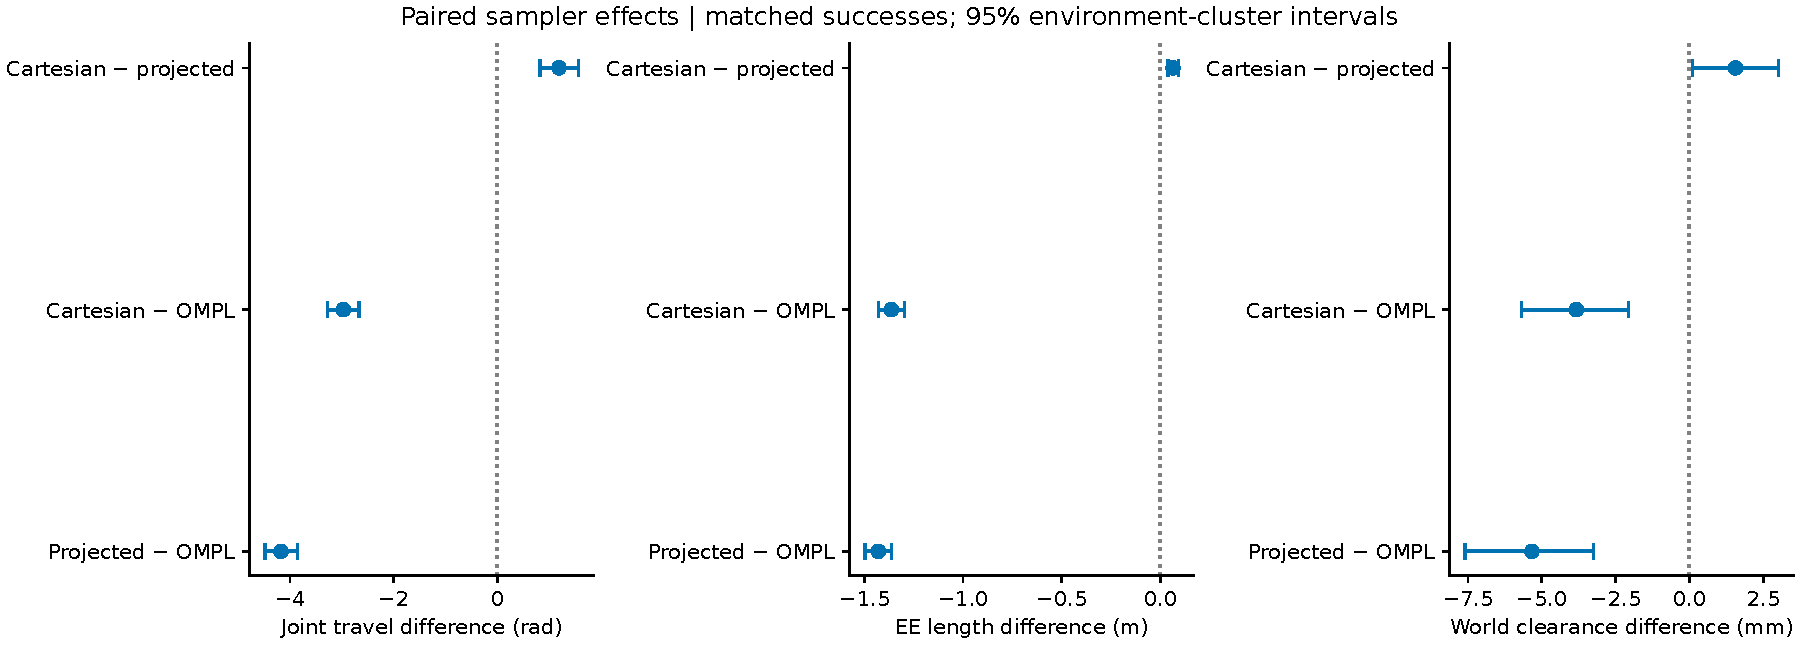
\includegraphics[width=\linewidth]{figures/paired_sampler_effects.pdf}
\caption{Paired path-quality effects. Differences are first method minus second, with pointwise 95\% environment-cluster intervals on matched successful requests. Negative length differences favor the first method; positive clearance differences favor the first method. Intervals are not adjusted for the 24-test family.}
\end{figure}

The runtime results distinguish inexpensive online proposals from total planning cost. Joint projection required a median \textbf{21.775 ms} of sampler setup, largely anchor IK, followed by \textbf{0.165 ms} of online sampling per request. Cartesian + IK required \textbf{0.024 ms} of setup and \textbf{9.311 ms} of online sampling, including \textbf{9.065 ms} of online IK. The corresponding means differ from the medians because difficult requests produce long tails. There was no corrected difference between the two GMM methods in action latency, attributed pipeline latency or failure-penalized time. PAR2 assigned each failure 6 s and capped successful action times at the 3 s budget; the Cartesian-minus-projected PAR2 difference was −22.57 ms (95\% CI −56.56 to 5.51; adjusted \(p=1.0\)).

Cartesian + IK reduced action latency relative to unrestricted OMPL by 16.31 ms (95\% CI 11.27--21.44; adjusted \(p<0.001\)). This advantage did not extend to the full attributed pipeline. Shared model loading, TP-GMM reproduction, RL deformation and deformed GMR required mean core times of 6.007, 11.249, 2.033 and 2.429 ms, respectively. For each GMM request, pipeline latency adds the measured shared per-environment deformation-service wall time to request preparation/preflight and action latency. It is an attribution of preparation cost, not a separate deformation execution on every repeat; common endpoint IK and offline path auditing are excluded. With this accounting, Cartesian + IK was 10.92 ms slower than OMPL (95\% CI 5.68--16.04; adjusted \(p=0.0039\)), and projection was 18.97 ms slower (95\% CI 6.32--35.43; adjusted \(p=0.0391\)).

Cartesian + IK had a higher valid-proposal fraction: the equal-environment mean acceptance was \textbf{57.13\%} (95\% CI 55.36--58.96), compared with \textbf{20.74\%} (95\% CI 19.85--21.67) for projection. Aggregating all proposal counts instead gives 53.47\% and 12.98\%, respectively, illustrating the influence of difficult requests. Projection rejects proposals lacking anchors or violating trust-region, linearization, support, bounds or collision conditions. Its lower acceptance therefore does not directly imply greater sampling time: local draws and rejection tests can be much cheaper than repeated IK. These counters measure sampler returns, not RRT-tree insertions or all planner collision checks; corresponding internal counters were unavailable for unrestricted OMPL.

\begin{figure}
\centering
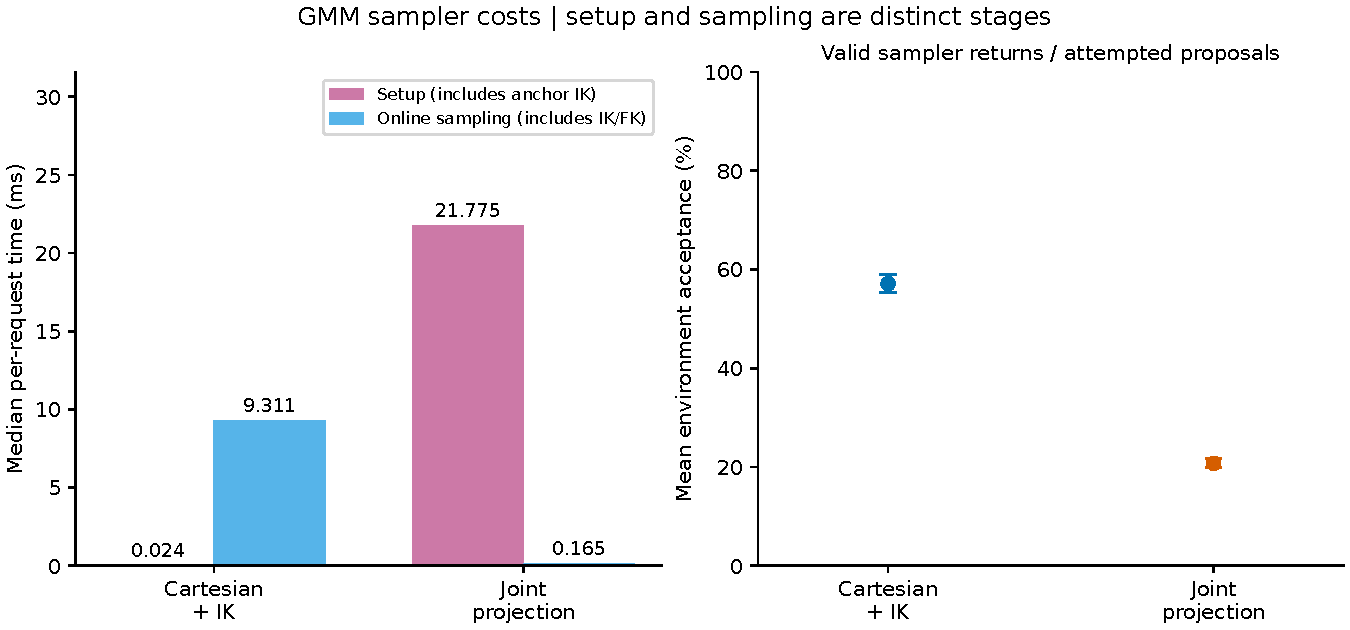
\includegraphics[width=\linewidth]{figures/sampler_costs.pdf}
\caption{GMM sampler costs. Left: descriptive per-request median setup and online-sampling times, shown separately. Right: equal-environment mean valid-proposal fraction with 95\% cluster intervals. Setup and sampling include nested IK/FK timers; these must not be added again.}
\end{figure}

\hypertarget{discussion-and-sampler-choice}{%
\subsection{Discussion and sampler choice}\label{discussion-and-sampler-choice}}

Cartesian + IK offers a direct connection between the learned spatial mixture and pre-IK targets, negligible sampler setup, and higher proposal acceptance in this experiment. Its principal cost is repeated online IK. IK solution selection and validity filtering still modify the accepted robot-state distribution, and a fixed positional proposal does not determine a unique joint configuration. It is an attractive option when transparent Cartesian proposal behavior and minimal anchor preparation are priorities.

Joint projection shifts IK work into anchor preparation and subsequently uses inexpensive local joint-space proposals. Its observed advantage was shorter unsimplified joint and end-effector paths, rather than demonstrated superiority in reliability or total latency. Its limitations include anchor coverage, singularity handling, trust-region and linearization restrictions, lower proposal acceptance and approximate task-space fidelity. Position-null-space exploration also changes tool orientation. These restrictions can matter when transferring to tight disassembly motions or introducing orientation constraints, but that transfer has not been tested here.

Unrestricted OMPL provides a model-independent reference that can explore beyond the learned corridor. It had complete observed success, lower attributed pipeline latency and greater measured robot-to-world clearance in this scene family, at the cost of substantially longer unsimplified paths. No pairwise success or PAR2 advantage was established after correction. Its larger allowed region and absence of model preparation are part of this comparison, rather than controlled-away implementation details.

Taken together, the results support \textbf{joint projection as the provisional GMM sampler for the subsequent benchmark when path compactness is the selection criterion}. They do not justify a general claim that it plans faster or more reliably than Cartesian + IK. This choice should be fixed before evaluation on independent EV disassembly scenes. The present evidence is limited to one robot, a table-and-cylinder scene family, a fixed learned model and policy, strict GMM guidance without fallback, unsimplified RRTConnect paths and the stated time budget; it does not establish transfer to the later benchmark or general superiority across planning tasks.
